% !TEX TS-program = XeLaTeX
% use the following command:
% all document files must be coded in UTF-8
\documentclass[portuguese]{textolivre}
% build HTML with: make4ht -e build.lua -c textolivre.cfg -x -u article "fn-in,svg,pic-align"

\journalname{Texto Livre}
\thevolume{15}
%\thenumber{1} % old template
\theyear{2022}
\receiveddate{\DTMdisplaydate{2022}{4}{15}{-1}} % YYYY MM DD
\accepteddate{\DTMdisplaydate{2022}{6}{7}{-1}}
\publisheddate{\DTMdisplaydate{2022}{8}{1}{-1}}
\corrauthor{Daiane Padula Paz}
\articledoi{10.35699/1983-3652.2022.39263}
%\articleid{NNNN} % if the article ID is not the last 5 numbers of its DOI, provide it using \articleid{} commmand 
% list of available sesscions in the journal: articles, dossier, reports, essays, reviews, interviews, editorial
\articlesessionname{articles}
\runningauthor{Paz et al.} 
%\editorname{Leonardo Araújo} % old template
\sectioneditorname{Bárbara Amaral da Silva}
\layouteditorname{Carolina Garcia}

\title{Competência digital docente: uma revisão de literatura}
\othertitle{Digital teaching competence: a literature review}
% if there is a third language title, add here:
%\othertitle{Artikelvorlage zur Einreichung beim Texto Livre Journal}

\author[1,2]{Daiane Padula Paz \orcid{0000-0003-2658-9426} \thanks{Email: \href{mailto:daippaz@gmail.com}{daippaz@gmail.com}}}
\author[3]{Edilson Pontarolo \orcid{0000-0002-6382-6403} \thanks{Email: \href{mailto:epontarolo@utfpr.edu.br}{epontarolo@utfpr.edu.br}}}
\author[1]{Franciele Clara Peloso \orcid{0000-0002-9647-001X} \thanks{Eamail: \href{mailto:clara@utfpr.edu.br}{clara@utfpr.edu.br}}}
\affil[1]{Universidade Tecnológica Federal do Paraná, Programa de pós-graduação em Desenvolvimento Regional, Pato Branco, PR, Brasil.}
\affil[2]{Instituto Federal do Paraná, Palmas, PR, Brasil.}
\affil[3]{Universidade Tecnológica Federal do Paraná, Departamento Acadêmico de Informática e Programa de Pós-Graduação em Desenvolvimento Regional, Pato Branco, PR, Brasil.}

\addbibresource{article.bib}
% use biber instead of bibtex
% $ biber article

% used to create dummy text for the template file
\definecolor{dark-gray}{gray}{0.35} % color used to display dummy texts
\usepackage{lipsum}
\SetLipsumParListSurrounders{\colorlet{oldcolor}{.}\color{dark-gray}}{\color{oldcolor}}

% used here only to provide the XeLaTeX and BibTeX logos
\usepackage{hologo}

% if you use multirows in a table, include the multirow package
\usepackage{multirow}

% provides sidewaysfigure environment
\usepackage{rotating}

% CUSTOM EPIGRAPH - BEGIN 
%%% https://tex.stackexchange.com/questions/193178/specific-epigraph-style
\usepackage{epigraph}
\renewcommand\textflush{flushright}
\makeatletter
\newlength\epitextskip
\pretocmd{\@epitext}{\em}{}{}
\apptocmd{\@epitext}{\em}{}{}
\patchcmd{\epigraph}{\@epitext{#1}\\}{\@epitext{#1}\\[\epitextskip]}{}{}
\makeatother
\setlength\epigraphrule{0pt}
\setlength\epitextskip{0.5ex}
\setlength\epigraphwidth{.7\textwidth}
% CUSTOM EPIGRAPH - END

% LANGUAGE - BEGIN
% ARABIC
% for languages that use special fonts, you must provide the typeface that will be used
% \setotherlanguage{arabic}
% \newfontfamily\arabicfont[Script=Arabic]{Amiri}
% \newfontfamily\arabicfontsf[Script=Arabic]{Amiri}
% \newfontfamily\arabicfonttt[Script=Arabic]{Amiri}
%
% in the article, to add arabic text use: \textlang{arabic}{ ... }
%
% RUSSIAN
% for russian text we also need to define fonts with support for Cyrillic script
% \usepackage{fontspec}
% \setotherlanguage{russian}
% \newfontfamily\cyrillicfont{Times New Roman}
% \newfontfamily\cyrillicfontsf{Times New Roman}[Script=Cyrillic]
% \newfontfamily\cyrillicfonttt{Times New Roman}[Script=Cyrillic]
%
% in the text use \begin{russian} ... \end{russian}
% LANGUAGE - END

% EMOJIS - BEGIN
% to use emoticons in your manuscript
% https://stackoverflow.com/questions/190145/how-to-insert-emoticons-in-latex/57076064
% using font Symbola, which has full support
% the font may be downloaded at:
% https://dn-works.com/ufas/
% add to preamble:
% \newfontfamily\Symbola{Symbola}
% in the text use:
% {\Symbola }
% EMOJIS - END

% LABEL REFERENCE TO DESCRIPTIVE LIST - BEGIN
% reference itens in a descriptive list using their labels instead of numbers
% insert the code below in the preambule:
%\makeatletter
%\let\orgdescriptionlabel\descriptionlabel
%\renewcommand*{\descriptionlabel}[1]{%
%  \let\orglabel\label
%  \let\label\@gobble
%  \phantomsection
%  \edef\@currentlabel{#1\unskip}%
%  \let\label\orglabel
%  \orgdescriptionlabel{#1}%
%}
%\makeatother
%
% in your document, use as illustraded here:
%\begin{description}
%  \item[first\label{itm1}] this is only an example;
%  % ...  add more items
%\end{description}
% LABEL REFERENCE TO DESCRIPTIVE LIST - END


% add line numbers for submission
%\usepackage{lineno}
%\linenumbers

\begin{document}
\maketitle

\begin{polyabstract}
\begin{abstract}
Este artigo tem por objetivos realizar uma revisão da literatura sobre Competência Digital Docente para composição de um portfólio referencial de produções científicas relevantes; caracterizar o estado do conhecimento sobre esse tema por meio da análise sistêmica do portfólio levantado e identificar oportunidades de pesquisas sobre Competência Digital Docente. Para tanto, utilizou-se o método ProKnow-C, o qual, por intermédio de critérios definidos em suas etapas, permitiu selecionar um portfólio bibliográfico de referências de destaque na literatura internacional, oriundas das bases de dados \textit{Web of Science e Scopus}. O referido portfólio resultou em 47 artigos relevantes sobre Competência Digital Docente, os quais foram submetidos a análises bibliométrica e sistêmica. Os resultados permitiram obter uma visão holística e profunda sobre o objeto de pesquisa, identificando o reconhecimento científico do material mediante fatores de impacto, autores especialistas sobre o tema, sua filiação institucional, teor das pesquisas, bem como lacunas e oportunidades de estudos futuros.

\keywords{Competência Digital Docente \sep Educação \sep Revisão de literatura \sep Proknow-C}
\end{abstract}

\begin{english}
\begin{abstract}
This article aims to: conduct a literature review on Digital Teaching Competence to compose a reference portfolio of relevant scientific productions; characterize the state of knowledge on this topic through the systemic analysis of the surveyed portfolio; identify research opportunities on Digital Teaching Competence. For this purpose, the ProKnow-C method was used, which allowed through criteria defined in its stages, the selection of a bibliographic portfolio of prominent references in the international literature from the Web of Science and Scopus databases. This portfolio resulted in 47 relevant articles on Digital Teaching Competence, which were submitted to bibliometric and systemic analysis. The results allowed a holistic and in-depth view of the research object, identifying scientific recognition of the material through impact factors, expert authors on the subject, their institutional affiliation, gaps in research, as well as opportunities for future studies.

\keywords{Digital Teaching Competence \sep Education \sep Literature review \sep Proknow-C}
\end{abstract}
\end{english}
% if there is another abstract, insert it here using the same scheme
\end{polyabstract}

\section{Introdução}

O crescente desenvolvimento e expansão das Tecnologias Digitais de Informação e Comunicação tem gerado mudanças em diversos setores da sociedade, tais como saúde, educação, segurança, economia, entre outros. Essas modificações são tão profundas, que requerem dos usuários destas tecnologias um rol de competências, denominadas \textit{competências digitais}.

No caso da Educação, a competência do professor para uso das Tecnologias da Informação e Comunicação no contexto profissional, com bom critério didático-pedagógico e que contribui para a formação digital de seus alunos, é denominada Competência Digital Docente \cite{espinosa__competencia_2018,pettersson_issues_2018,spante_digital_2018}. Devido a sua importância, tem ganhado destaque em políticas governamentais de diversos países e em pesquisas na área da Educação, as quais têm gerado, nos últimos anos, uma diversidade de \textit{frameworks}, propostas e nomenclaturas, constituindo um arcabouço sobre o tema.

Considerando tais aspectos, idealizou-se este estudo, que tem por objetivos: 
a) realizar uma revisão da literatura sobre Competência Digital Docente (CDD), para composição de um portfólio referencial de produções científicas relevantes;
b) caracterizar o estado do conhecimento sobre CDD por meio da análise sistêmica do portfólio bibliográfico levantado e; 
c) identificar oportunidades de pesquisa sobre o tema.

Metodologicamente, a presente pesquisa é definida como \textit{bibliográfica por revisão abrangente de literatura}, efetivada a partir do método \textit{Knowledge Development Process-Contructivist} (ProKnow-C) \cite{ensslin_proknow-c_2010}, cujos procedimentos estão descritos de maneira detalhada ao longo do artigo, compondo suas seções. O método selecionado permitiu obter um conjunto de referências de destaque na literatura acadêmica, bem como empreender análises profundas, que conformaram o estado do conhecimento sobre o tema \textit{Competência Digital Docente} e, por conseguinte, elencar oportunidades de pesquisas futuras.

Esse texto está organizado em quatro grandes seções, a saber: introdução, que apresenta brevemente o artigo; metodologia, que descreve os procedimentos do método adotado, incluindo detalhamento de busca nas bases de dados, seleção do portfólio bibliográfico e análise bibliométrica; resultados, que descreve e discute os achados a partir da análise sistêmica e identificação de oportunidades de pesquisa; e, por fim, conclusão, que encerra com limitações e relevância do estudo empreendido. 

\section{Metodologia}

Definida metodologicamente como \textit{revisão abrangente de literatura}, esta pesquisa mapeia o conhecimento produzido na literatura científica e sintetiza o que se sabe sobre o tema \cite{yin_pesquisa_2016}. Para tanto, foi utilizado o método ProKnow C \cite{ensslin_proknow-c_2010}, selecionado por seguir um protocolo que atende aos objetivos determinados e porque, segundo \textcite[p.~56]{linhares_capacidade_2019}, “possibilita ao pesquisador reunir um portfólio com reconhecimento científico e relevância ao tema de interesse”.

O ProKnow C está alinhado a uma abordagem qualitativa construtivista, cujo interesse é gerar conhecimento e intervir cientificamente a partir da seleção e da análise crítica de material bibliográfico publicado. Este método propõe quatro etapas sistemáticas, a saber: (i) seleção de portfólio; (ii) análise bibliométrica; (iii) análise sistêmica; e (iv) identificação de oportunidades de pesquisa.

\subsection{Etapa 1: Seleção do Portfólio Bibliográfico}

O método indica que os temas de pesquisa sejam pensados a partir de eixos, sendo, nesse caso: eixo 1, a competência digital; e eixo 2, docente. Em cada eixo, foram definidas palavras-chave e operadores booleanos, testados por aderência, resultando na seguinte expressão lógica utilizada como parâmetro no comando de busca: \textit{(("digital competenc*" OR "digital skill*" OR "digital literac*")) AND (("teach*" OR "educat*" OR "professor"))}. A partir dessa sentença de busca, foram eleitas as bases de dados que forneceram maior quantidade de resultados, \textit{Web of Science} e a \textit{Scopus}, bases internacionais abrangentes e relevantes na área multidisciplinar.

Os procedimentos, os resultados de buscas e a composição dos bancos de dados estão detalhados a seguir.

\subsubsection{Resultados de buscas na base \textit{Web Of Science}}

A busca nesta base resultou em 3128 publicações. Ao analisar o período, notou-se que a primeira publicação surge em 1997 e começa a se intensificar a partir de 2010, ano que teve 55 referências publicadas. Considerando os quantitativos de 2010 e os de 2020, percebe-se que houve um aumento de 621\% de publicações, o que denota um importante crescimento de interesse científico pelo tema.

Na sequência, foram sendo aplicados filtros para seleção de resultados desejados. Primeiramente, delimitou-se o escopo, o qual teve como período publicações do tipo artigo entre 2010 e 2020, nos idiomas inglês, espanhol e português. Foram excluídas as categorias da área da Saúde e não se aplicou nenhuma restrição quanto ao país de publicação. Estes critérios resultaram em 864 referências que compuseram o Banco de Dados Brutos 1 (BDB1) deste estudo.

\subsubsection{Resultados de buscas na base \textit{Scopus}}

A busca na base \textit{Scopus}, com a mesma expressão lógica descrita na seção anterior, resultou em 3291 documentos. A primeira publicação sobre o tema também aparece no ano de 1997, porém ao se comparar a disponibilidade de referências nesta base com a \textit{Web of Science}, notou-se que, embora tenha havido crescimento anual de publicações, houve menores quantidades de publicações nos anos de 2015 a 2019.

Posteriormente, foram sendo aplicados critérios de exclusão por meio de filtros disponíveis, procurando manter o máximo de equidade com os aplicados na anterior. O primeiro critério foi a delimitação temporal (período de 2010 a 2020); o segundo, foi a exclusão de áreas relacionadas à Saúde, à Economia, à Astronomia, à Engenharia e à Biologia. Também foram delimitados os idiomas de publicação com maiores quantitativos − inglês, espanhol e português −, o tipo de acesso aberto, e não se aplicou nenhuma restrição referente a país de publicação. Estes procedimentos resultaram em 599 documentos, que compuseram o Banco de Dados Brutos 2 (BDB2) deste estudo.

\subsubsection{Tratamento do Banco de Dados Brutos Unificado}

Foram selecionados, nas duas bases pesquisadas, os seguintes dados para exportação em planilha Microsoft Excel: título, autores, revista, ano de publicação, \textit{Digital Object Identifier} (DOI) e total de citações. Criou-se a Planilha 1, correspondente ao BDB1, com 864 títulos oriundos da \textit{Web of Science}, e a Planilha 2, correspondente ao BDB2, com 599 títulos oriundos da \textit{Scopus}. Os metadados exportados a partir das bases não eram uniformes, nem completos, o que exigiu uma minuciosa revisão e busca complementar para a elaboração da Planilha 3 (BDBU), que unificou 1463 referências. Nesta etapa, foram excluídos 340 títulos duplicados, restando 1123 referências na segunda versão do BDBU, as quais foram exportadas para o \textit{software Mendeley} para as operações posteriores.

Passou-se à leitura dos títulos para verificar se estavam alinhados ao tema CDD e criou-se um sistema de notas para classificação, sendo que 0 representa “nada relevante” para este estudo, 1 representa “pouco relevante”, e 2, “muito relevante”. Os 801 artigos que receberam nota 0 foram excluídos; os 169 que receberam nota 1 foram deixados para pesquisas futuras; e os 153 que receberam nota 2 passaram para a etapa 2 do método ProKnow C, que consiste na análise bibliométrica para seleção de portfólio.

\subsection{Etapa 2: Análise Bibliométrica para seleção do portfólio bibliográfico}

A primeira análise realizada nos 153 artigos selecionados foi o número de citações. Para tanto, realizou-se buscas no \textit{Google Scholar}, considerado como fonte uniforme. Logo, as referências foram listadas em ordem decrescente pelo número de citações e aplicou-se o princípio de Pareto, critério comumente usados neste método, que preconiza que 80\% de um efeito é explicado por 20\% das causas. Nesse caso, 80\% das contagens de citações são derivadas de 20\% das publicações \cite{de_carvalho_bibliometrics_2020}.

Nesse portfólio, o artigo mais citado recebeu 131 citações, correspondendo a 5\% do total (2629 citações), e o artigo que alcançou 80\% de representatividade (R) tem 21 citações, sendo essa a linha de corte fixada, justificando o Princípio de Pareto. Assim, 43 artigos foram selecionados como relevantes por seus índices de citações, o que significa 28,10\% do total de 153 artigos da lista. Na sequência do método, indica-se a leitura dos resumos das referências, para classificá-las como alinhadas ou não ao tema \cite{linhares_capacidade_2019}, o que permitiu excluir seis referências, restando 37, que compuseram o Repositório A.

Notou-se que, das 153 referências selecionadas na Etapa 1, mais da metade (81) foi publicada nos últimos dois anos – 38 em 2019 e 43 em 2020. Embora, na aplicação do Princípio de Pareto, cinco artigos recentes foram incluídos (todos do ano de 2019); preciso, portanto, considerar outros critérios de inclusão ou exclusão desse tipo de referência, pois, por serem publicações recentes, não tiveram tempo hábil para acumular citações. Para esses casos, o método sugere a leitura dos resumos para exclusão dos que não sejam alinhados ao tema de interesse. Assim, dos 76 artigos com publicação recente, 28 foram excluídos, restando 48 (21 publicados em 2019 e 27 em 2020), que compuseram parte do Repositório B.

Ainda, para formação do Repositório B, foi realizado o procedimento de repescagem de publicações. Para isso, fez-se uma lista com os nomes de todos os autores e coautores dos 43 artigos selecionados pelo Princípio de Pareto (Lista de Autores 1, contendo 95 nomes) e, à parte, uma lista com os autores dos 34 artigos que não eram nem recentes, nem selecionados via Princípio de Pareto (Lista de Autores 2, contendo 79 nomes). Comparou-se as listas e identificou-se aqueles que coincidiam em ambas, sendo, neste caso, sete autores, com seis publicações ao todo. Realizou-se, também, a leitura desses resumos, e excluiu-se uma referência, mantendo-se as outras cinco no Repositório B.

Seguindo o método, procedeu-se à elaboração do Repositório C, o qual foi composto pelas referências do Repositório B (53 referências, sendo 48 publicadas recentemente e cinco selecionadas na repescagem) e do Repositório A (37 referências selecionadas por sua representatividade em função da quantidade de citações), totalizando 90 documentos. Sequencialmente, foi realizada a leitura completa de cada artigo e aplicou-se um parâmetro de seleção, elaborado pelos pesquisadores, considerando quatro categorias de interesse, a saber: Categoria 1 – Apresenta conceitos sobre CD, CDD, LD e/ou \textit{review}; Categoria 2 – Apresenta \textit{frameworks} para o desenvolvimento e/ou resultados de avaliação de CDD; Categoria 3 – Apresenta propostas e/ou discussões sobre formação da CDD; Categoria 4 – Apresenta modelos de certificação de CDD. Foram excluídas todas as referências que não atendiam os critérios estabelecidos nas categorias, restando, portanto, 47 que formaram o portfólio bibliográfico desta pesquisa, apresentado na \Cref{Table1}:

\begin{table}[h!]
\centering
\begin{threeparttable}
\caption{Portfólio bibliográfico obtido a partir do método Proknow-C.}
\label{Table1}
\begin{tabular} {lp{0.5\textwidth}}
\toprule
CATEGORIA & REFERÊNCIA \\
\midrule
\arrayrulecolor[gray]{.7}
\multirow{4}{*}{CAT1: DEFINIÇÃO 13 referências} &
\textcite{granados_competencias_2020,engen_comprendiendo_2019,falloon_digital_2020,gutierrez_media_2012,park_scientometric_2020,perez_competencia_2012,pettersson_issues_2018,espinosa__competencia_2018,reddy_digital_2020,garcia_impacto_2019,spante_digital_2018,stordy_taxonomy_2015,villa_competencias_2019} \\
\midrule 
\multirow{7}{*}{CAT2: AVALIAÇÃO 28 referências} & 
\textcite{ata_exploring_2019,andrade_digital_2020,botturi_digital_2019,_almenara_tic_2019,almenara_marco_2020,caena_aligning_2019,cebi_digital_2020,bravo_development_2019,trindade_assessment_2020,trindade_escala_2019,coscollola_fomentando_2020,boudet_evaluacion_2017,marquez_competencias_2018,cuartero_alisis_2016,flores_practica_2020,repiso_alisis_2016,escudero_alisis_2019,lucena_factors_2019,cantabrana_evaluacion_2019,revilla_assessing_2020,ruiz_profesorado_2016,hernandez_evolucion_2020,diaz_competencia_2019,sanchez_alisis_2020,cabezas_university_2020,quiroz_indicadores_2016,tsankov_digital_2019,viberg_validating_2020} \\
\midrule
\multirow{2}{*}{CAT3: FORMAÇÃO 5 referências} & 
\textcite{rosenblit_e-teaching_2018,hepp_teacher_2015,instefjord_appropriation_2015,gomez_formacion_2019,trigueros_digital_2019} \\
\midrule
CAT4: CERTIFICAÇÃO 1 referência & \textcite{cuartero_certificacion_2019} \\
\arrayrulecolor{black}
\bottomrule
\end{tabular}
\source{Dados da pesquisa.}
\end{threeparttable}
\end{table}

Visando conhecer mais profundamente os dados do portfólio, foi realizada uma análise bibliométrica do material selecionado, a qual diz respeito à relevância dos periódicos e de suas referências, e ao cruzamento dos periódicos com o referencial \cite{ensslin_processo_2013}. Para tanto, foi organizada uma lista com todos os periódicos e com o número de publicações do portfólio em cada uma. (\Cref{Figura01}).

\begin{figure}[htbp]
\centering
\caption{Índice SNIP e quantidade de publicações por revista no portfólio selecionado.}
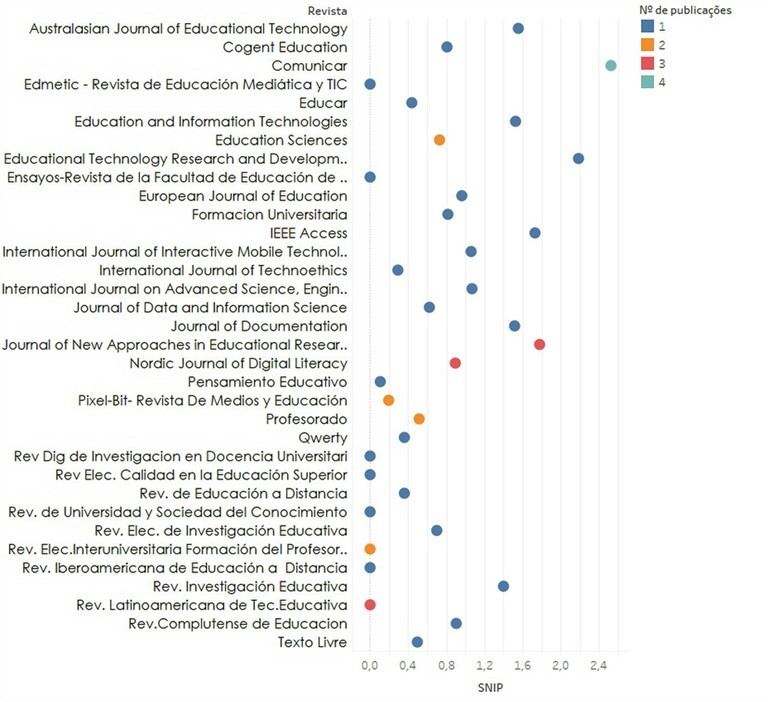
\includegraphics[width=0.9\textwidth]{figura01.png}
\label{Figura01}
\source{Dados da pesquisa.}
\end{figure}

Buscou-se, ainda, seus índices de \textit{Source Normalized Impact per Paper} (SNIP), fator que estabelece uma razão entre o número médio de citações por artigo e o potencial de citação da área do conhecimento a que se refere o periódico, na base \textit{CWTS Journal Indicators}, a fim de observar possíveis relações entre estas variáveis 

A segunda análise realizada foi referente à quantidade de publicações por ano no portfólio (\Cref{Figura02}).

\begin{figure}[htbp]
\centering
\caption{Quantidade de publicações por ano no portfólio selecionado.}
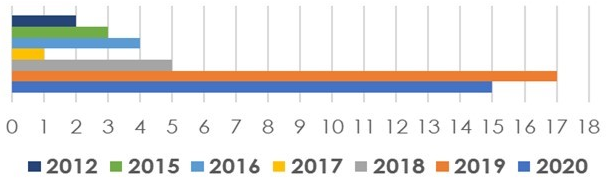
\includegraphics[width=0.8\textwidth]{figura02.png}
\label{Figura02}
\source{Dados da pesquisa.}
\end{figure}

Os dados revelam que, entre os 47 artigos, 32 foram publicados nos anos 2019 e 2020, ou seja, 68\% do \textit{corpus} selecionado, o que indica que essa temática vem sendo endereçada por um maior número de pesquisas nos últimos anos. Quanto ao reconhecimento científico do material, observou-se que tiveram maiores índices de citações no Google Scholar as seguintes referências: \textcite{gutierrez_media_2012}, com 123 citações, e \textcite{perez_competencia_2012}, com 112 citações, ambos publicados na Revista Comunicar. Também se destacam \textcite{pettersson_issues_2018}, com 85 citações, e \textcite{spante_digital_2018}, com 70. Esses dados permitem reconhecer os estudos seminais, nesse caso, publicados em 2012, e os estudos recentes, que são também importantes, por já possuírem expressivos números de citações.

Buscando saber quem são os especialistas sobre o tema, realizou-se uma lista com todos os autores e coautores dos artigos do portfólio e percebeu-se que alguns estão presentes em mais de uma publicação, demonstrando produtividade e interesse sobre a CDD. Para conhecer o perfil desses autores e seus impactos na academia, buscou-se no Google Scholar os fatores de impacto de produções (índices H e I10) e as instituições às quais estavam vinculados no momento dessa pesquisa (\Cref{Table02}).

\begin{table}[h!]
\centering
\begin{threeparttable}
\caption{Total de citações, afiliação e índices H e I10 dos autores do portfólio.}
\begin{tabular}{p{0.25\textwidth}p{0.1\textwidth}p{0.1\textwidth}p{0.1\textwidth}p{0.1\textwidth}p{0.22\textwidth}}
\toprule
Autor & Publicações no portfólio & Citações Scholar & Índice H &	Índice I10 & Instituição \\
\midrule
Almenara, Julio Cabero & 02 & 30186 & 84 & 370 & Universidad Sevilla \\
Espinosa, María Paz Prendes & 03 & 7444 & 36 & 112 & Universidad de Murcia \\
Cervera, Mercè Gisbert & 02 & 6122 & 40 & 104 & Universitat Rovira i Vigili \\
Porlán, Isabel Gutiérrez & 03 & 2210 & 18 & 28 & Universidad de Murcia \\
Moreira, José Antonio & 02 & 1795 & 22 & 49 & Universidade Aberta Portugal \\
Torres, Juan Manuel Trujillo & 02 & 385 & 22 & 18 & Universidad de Granada \\
Trigueros, Isabel Gómz & 02 & 423 & 10 & 11 & Universidad de Alicante \\
Sánchez, Delfín Ortega & 02 & 405 & 10 & 10 & Universidad Burgos\\
Thevenet, Paula Sánchez & 02 & 304 & 8 & 6 & Universidad Cardenal Herrera \\
Cuartero, Marta Durán & 02 & 288 & 5 & 4 & Universidad Murcia \\
Bellido, María Rosario García & 02 & 158 & 7 & 6 & Universidad Cardenal Herrera \\
Bañuls, Mónica Ruiz & 02 & 112 & 5 & 3 & Universidad de Alicante \\
Trindade, Sara Días & 02 & 73 & 5 & 0 & Universidade de Coimbra \\
Gómez, Beatriz Lores & 02 & 13 & 2 & 0 & Universidad Cardenal Herrera \\
\bottomrule
\end{tabular}
\source{Dados da pesquisa.}
\label{Table02}
\end{threeparttable}
\end{table}

Nota-se que, entre os catorze autores listados, oito possuem $I10\geqslant10$ e $H\geqslant10$. Nesse escopo, o autor com maior destaque em todas as categorias de fator de impacto foi Julio Cabero Almenara, cujo número de citações excedem trinta mil, seguido por María Paz Prendes Espinosa, citada mais de sete mil vezes.

\section{Resultados}

As etapas três e quatro do método Proknow-C, que são análise sistêmica e identificação de oportunidades de pesquisa, as quais estão descritos a seguir, representam os resultados obtidos nesse estudo.

\subsection{Etapa 3: Análise Sistêmica}

Para análise sistêmica do Portfólio, realizou-se a importação dos arquivos na íntegra para o \textit{software} de análise de dados \textit{Atlas.ti}, versão 9, os quais foram organizados conforme as categorias apresentadas no Quadro 3. Criou-se, nesse mesmo \textit{software}, códigos que representam os itens de interesse sobre o objeto de estudo, determinados no método ProKnow C como lentes metodológicas ou de análise \cite{ensslin_proknow-c_2010,linhares_capacidade_2019}.

A primeira lente de análise foi a contextual, ou seja, o levantamento dos locais em que as pesquisas foram aplicadas e dos sujeitos envolvidos. A segunda lente focou no teor dos estudos, analisando, por meio dos objetivos, da abordagem e/ou da metodologia utilizados, quais têm sido os aspectos estudados acerca da CDD. A terceira lente foi a de evidências e de lacunas destacadas nos estudos, de modo a conformar o estado do conhecimento sistematizado e demarcar pontos essenciais para a última fase do método, que é a identificação de oportunidades de pesquisa.

\subsubsection{Análise contextual}

Pela análise contextual, observou-se que o universo das pesquisas se limitou a instituições de ensino de nível secundário e de ensino superior, em diferentes continentes: América (Chile, Colômbia, Costa Rica, Equador, México, República Dominicana, Uruguai); Europa (Bulgária, Espanha, França, Noruega, Portugal, Suécia, Suíça); Ásia (Coreia do Sul), e Eurásia (Turquia). Cabe agregar que, nesse portfólio, a Espanha é o país com maior número de pesquisas aplicadas em seu território (treze referências), sendo algumas de abrangência regional nas Comunidades Autônomas, como Aragão, Andaluzia e Catalunha, e outras com prospecção local, como Alicante, Burgos, Málaga, Múrcia e Valladolid.

Pela mesma análise, foram identificados os sujeitos das pesquisas, que são professores e estudantes em formação docente. Nesse sentido, os autores demonstraram preocupação sobre como desenvolver a CDD daqueles que estão ascendendo à docência, uma vez que grande parte dos professores formadores advém de uma geração menos tecnológica; além disso, muitas instituições que proveem essa formação, não contemplam a CDD em seus currículos.

\subsubsection{Teor das pesquisas sobre CDD}

Para compreender teor das pesquisas analisadas, realizou-se uma leitura informativa, a qual visou a coleta de informações para determinado propósito \cite{lakatos_fundamentos_2003}, ou seja, buscou-se quais aspectos relacionados à CDD têm sido objeto de estudo e quais os procedimentos metodológicos aplicados. A \Cref{Table03} apresenta, de forma sintética, as análises feitas sob a segunda lente.

\begin{table}[h!]
\centering
\begin{threeparttable}
\caption{Teor das pesquisas sobre CDD em quatro categorias.}
\label{Table03}
\begin{tabular}{p{1.0\textwidth}}
\hline
Categoria 1 – Definição (13 referências) \\
Pesquisas que buscam definir e/ou discutir conceitos sobre competência, CD, CDD e literacias. Dentro dessa categoria, foram identificadas três subcategorias:
\begin{enumerate}[label=\alph*.]
    \item Pesquisas realizadas com base em revisão de literatura sobre conceitos predominantes na academia ou para identificação de tendência de estudos realizados sobre o tema em um marco temporal. \textcite{falloon_digital_2020,pettersson_issues_2018,park_scientometric_2020,espinosa__competencia_2018,reddy_digital_2020,spante_digital_2018,stordy_taxonomy_2015,garcia_impacto_2019};
    \item Pesquisas realizadas com base em análise documental, buscando identificar antecedentes sobre competência digital no contexto educacional. \textcite{granados_competencias_2020, perez_competencia_2012};
    \item Pesquisas de discussão que tratam sobre as condições sociais e culturais implicadas no uso de TIC e as alfabetizações necessárias para o século XXI. \textcite{gutierrez_media_2012,engen_comprendiendo_2019,villa_competencias_2019}.
\end{enumerate} \\
\hline 
Categoria 2 – Avaliação (28 referências) \\
Pesquisas que apresentam ou discutem \textit{frameworks} para desenvolvimento e avaliação da CDD, bem como estudos de caso em diferentes realidades. Dentro dessa categoria, foram identificadas seis subcategorias:
\begin{enumerate}[label=\alph*.]
    \item Pesquisas que avaliam os níveis de CDD. \textcite{trindade_assessment_2020,boudet_evaluacion_2017,marquez_competencias_2018,flores_practica_2020,repiso_alisis_2016,escudero_alisis_2019,ruiz_profesorado_2016,diaz_competencia_2019,cabezas_university_2020,tsankov_digital_2019,hernandez_evolucion_2020};
    \item Pesquisas que analisam \textit{frameworks} para o desenvolvimento da CDD, divididas em três subgrupos:
    \begin{enumerate}
    \item \textit{Conjunto de modelos}.\textcite{cuartero_alisis_2016};
    \item \textit{Modelo TPACK}. \textcite{revilla_assessing_2020, _almenara_tic_2019};
    \item \textit{Modelo DigicompEdu}. \textcite{almenara_marco_2020,caena_aligning_2019}.
    \end{enumerate}
    \item Pesquisas que propõem um modelo de avaliação de CDD. \textcite{bravo_development_2019,cantabrana_evaluacion_2019,quiroz_indicadores_2016,trindade_escala_2019,viberg_validating_2020};
    \item Pesquisas que buscam identificar aspectos que incidem no nível de CDD, como:
    \begin{enumerate}
    \item \textit{Relações entre gênero e geração}. \textcite{andrade_digital_2020,cebi_digital_2020};
    \item \textit{Aspectos sociodemográficos}. \textcite{lucena_factors_2019};
    \item Fatores inerentes à função docente, como idade, sexo, formação e experiência laboral.\textcite{sanchez_alisis_2020}.
    \end{enumerate}
    \item Pesquisas que investigam percepções de CD de professores em formação inicial. \textcite{ata_exploring_2019,coscollola_fomentando_2020};
    \item Pesquisas que avaliam os impactos de uma formação em alfabetização digital e midiática proposta. \textcite{botturi_digital_2019}.
\end{enumerate}
\\
\hline 
Categoria 3 – Formação (5 referências) \\
Pesquisas que discutem sobre aspectos relacionados à formação da CD de docentes em exercício e/ou em formação. Nessa categoria, foram identificadas três subcategorias:
\begin{enumerate}[label=\alph*.]
    \item Pesquisas que discutem aspectos relacionados ao desenvolvimento digital de docentes e a relação com discentes. \textcite{rosenblit_e-teaching_2018,hepp_teacher_2015};
    \item Pesquisas que apresentam estudos de caso de práticas de uso de TIC e as dificuldades encontradas na formação. \textcite{instefjord_appropriation_2015};
    \item Pesquisas que apresentam estudos de caso de formação inicial docente relacionada à CD. \textcite{gomez_formacion_2019,trigueros_digital_2019}.
\end{enumerate}
\\
\hline 
Categoria 4 – Certificação (1 referência) \\
Estudo que apresenta uma revisão de modelos de certificação para competência digital docente e apresenta uma proposta. \textcite{cuartero_certificacion_2019}.
\\
\hline
\end{tabular}
\source{Dados da pesquisa.}
\end{threeparttable}
\end{table}

As referências destacadas na categoria 1 tiveram por finalidade a análise documental, a discussão sobre o tema e/ou a revisão de literatura. Nesses casos, o percurso metodológico predominante foi de abordagem qualitativa, com resultados descritivos que tratam tanto de conceitos consolidados, como literacia digital \cite{stordy_taxonomy_2015,reddy_digital_2020}, ou emergentes, como CDD \cite{spante_digital_2018,garcia_impacto_2019}. Discute-se a problemática das diferentes nomenclaturas relacionadas às habilidades digitais \cite{park_scientometric_2020}, bem como o dimensionamento das TIC e seu potencial de aplicação no âmbito educacional.

As referências elencadas na categoria 2 centraram-se no desenvolvimento e na avaliação da CDD (ou de futuros docentes), seja a partir de estudos de caso, evidenciando diferentes realidades, como República Dominicana \cite{diaz_competencia_2019}, Portugal \cite{trindade_assessment_2020}, Espanha \cite{boudet_evaluacion_2017,marquez_competencias_2018,repiso_alisis_2016,escudero_alisis_2019,ruiz_profesorado_2016}, México \cite{flores_practica_2020}, Equador \cite{cabezas_university_2020}, Bulgária \cite{tsankov_digital_2019}, seja na investigação de percepções de docentes e discentes \cite{ata_exploring_2019,coscollola_fomentando_2020} ou, ainda, aquelas que apresentam uma intersecção de fatores que incidem sobre o desenvolvimento da CD. Os resultados mostraram que, nos diferentes contextos, os níveis de competência digital são aquém do considerado ideal, mesmo nos casos dos docentes que entendem a importância das TIC no ensino \cite{cabezas_university_2020}.

Outros estudos desta categoria centraram-se em conhecer aspectos que podem incidir nos níveis de CDD, tais como gênero, geração, experiência laboral e aspectos sociodemográficos. Nesse sentido, \textcite{sanchez_alisis_2020} perceberam, em seu estudo aplicado, que mulheres são mais criativas para a elaboração de conteúdos digitais, enquanto homens se sobressaem na solução de problemas, e \textcite{andrade_digital_2020} revelaram que o nível de competências digitais independe do gênero, mas depende da geração. Por outro lado, \textcite{lucena_factors_2019} identificaram que a experiência docente é o fator sociodemográfico com maior impacto na aquisição de competências digitais, ou seja, quanto mais anos de experiência na profissão, maior a tendência de um nível de competência digital elevado. Com a mesma finalidade, porém baseada em uma metodologia biográfico-narrativa, está a pesquisa de \textcite{hernandez_evolucion_2020}, na qual, a partir de relatos de vida de docentes do México e da Espanha, foram elencados quatro conjuntos de fatores que foram cruciais para o desenvolvimento da CDD dos entrevistados.

Sob a mesma lente de análise e ainda na categoria dois, foram identificados estudos que propõem ou analisam \textit{frameworks} de desenvolvimento da CDD. Entre os modelos de maior destaque na literatura, e que, inclusive, servem de base para os modelos propostos, estão o \textit{Technological Pedagogical Content Knowledge} \cite{mishra_technological_2006}, conhecido como TPACK, e o \textit{European Framework for the Digital Competence of Educators} \cite{redecker_european_2017}, conhecido como \textit{DigCompEdu}. Sumariamente, \textcite{cuartero_alisis_2016} consideram que todos os modelos avaliados incluem as competências relacionadas às dimensões e agregam como competências específicas a capacidade de inovação e de exploração do potencial educacional das TIC.

Na terceira categoria, que trata sobre a formação da CDD, foram identificadas três subcategorias de pesquisa. A primeira subcategoria relaciona-se aos aspectos do desenvolvimento digital de docentes e discentes, em que \textcite{rosenblit_e-teaching_2018} ressalta a importância de definir claramente os papéis dos professores em ambientes de estudo \textit{on-line} e prover formação adequada para esse fim, enquanto \textcite{hepp_teacher_2015} reiteram a necessidade de atualização docente, uma vez que consideram as TIC como componentes dessa profissão. A segunda subcategoria apresenta a preocupação com as dificuldades encontradas na formação da CDD, reveladas por \textcite{instefjord_appropriation_2015}, como o conflito entre domínio e apropriação das tecnologias, entre o uso pessoal e educacional e, ainda, a resistência existente entre docentes para sua implementação na prática pedagógica. A terceira subcategoria direciona-se para a formação inicial, a qual é destacada por diversos autores como a maior necessidade e principal alternativa para o desenvolvimento da CDD. Nesse sentido, \textcite{trigueros_digital_2019} ratificam que é fundamental favorecer o uso das TIC nas instituições formadoras de docentes, de forma a se adequar às necessidades da educação do século XXI.

Ao relacionar o tema CDD com o desenvolvimento, pode-se afirmar que, de forma geral, os autores acreditam que as TIC têm modificado continuamente diversos âmbitos, entre eles o educacional; sendo uma oportunidade para mudar e transformar a educação, que tem se mostrado aquém ou desconectada das necessidades sociais dos sujeitos do século XXI \cite{coscollola_fomentando_2020,flores_practica_2020,hepp_teacher_2015,rosenblit_e-teaching_2018}. Para tanto, ratifica-se a necessidade da valorização dos docentes e o alinhamento de políticas públicas para atividades formativas diversas que possam desenvolver sua CD \cite{falloon_digital_2020,pettersson_issues_2018}.

Na quarta categoria dessa análise sistêmica, há somente um estudo. Trata-se da pesquisa empreendida por \textcite{cuartero_certificacion_2019}, que trazem uma revisão bibliográfica de algumas propostas de instrumentos de certificação da CD e, a partir de análises feitas e de estudos relacionados, perceberam a ausência de testes para certificação da CDD de professores universitários e apresentaram uma proposta para este fim.

\subsubsection{Evidências e lacunas}

A terceira e última lente utilizada se deteve nas evidências e nas lacunas destacadas pelos autores, de forma geral. A primeira evidência observada foi que a competência digital tem sido considerada, pelos autores, como uma necessidade do século XXI, uma vez que as TIC têm modificado totalmente a dinâmica de diversos âmbitos, incluindo negócios, serviços, cultura e relações humanas \cite{villa_competencias_2019}. A segunda evidência é a percepção do docente como figura essencial para o desenvolvimento da CD da população. Nesta perspectiva, os docentes são vistos como facilitadores do desenvolvimento da CD de seus estudantes \cite{trindade_escala_2019}. A terceira evidência é a variedade de iniciativas que têm sido elaboradas com o objetivo de estipular diretrizes para o uso das tecnologias no contexto educacional, sobretudo para desenvolvimento, formação e avaliação da CDD.

Com relação às lacunas identificadas pelo grupo de autores deste portfólio, destacam-se três: a primeira, refere-se à confusão terminológica que tange os termos \textit{competência, competência digital} e \textit{competência digital docente}; a segunda, à ausência de suporte teórico sobre o tema; e a terceira, à necessidade de formação específica para favorecer o desenvolvimento da CDD.

A primeira lacuna implica no entendimento conceitual de CDD, uma vez que a variedade de termos utilizados − como competência audiovisual, midiática, literacia ou letramento digital −, provocam uma celeuma na comunidade acadêmica. A segunda lacuna atinge o embasamento de pesquisas sobre o tema de CDD, já que não há afiliações teóricas declaradas na maioria dos artigos, exceto em \textcite{flores_practica_2020}, e em \textcite{engen_comprendiendo_2019}. A ausência de um enfoque pedagógico, que sirva de base teórica, é, inclusive, mencionada por \textcite{gutierrez_media_2012} e por \textcite{bravo_development_2019}, sendo considerada urgente. A última lacuna refere-se à necessidade de formação docente para o desenvolvimento de sua CD, tanto inicial quanto continuada. Nessa perspectiva, considera-se a importância de políticas educacionais para esse fim.

Feitas as análises a partir da apropriação da literatura, passa-se à etapa final desse estudo.

\subsection{Etapa 4: Identificação de oportunidades de pesquisa}

A última etapa do método Proknow-C refere-se à identificação de oportunidades de pesquisa. A partir da análise crítica do referencial emergido nesse escopo, extrai-se alguns questionamentos, que podem compor oportunidades de pesquisas futuras em linhas que abrangem Tecnologias e Educação, a saber:

\textit{Em uma perspectiva social}: A ausência ou pouco desenvolvimento da competência digital entre os discentes pode afetar as condições de aprendizado nos ambientes virtuais? Esse pode ser um fator que conduz à evasão escolar?

\textit{Em uma perspectiva educacional}: Os docentes percebem a Competência Digital como uma condição necessária para o bom exercício de sua profissão? Quais as dificuldades que sentem em seu cotidiano?

\textit{Em uma perspectiva de desenvolvimento}: Como é desenvolvida a Competência Digital Docente? Quais fatores incidem nesse processo?

A partir da leitura crítica de cada pesquisador, muitos outros questionamentos podem surgir, os quais podem relacionar a CDD a outras perspectivas, seja de ordem pessoal, cultural, econômica, e a diferentes áreas do saber, configurando novas ideias de pesquisa.

\section{Conclusão}

A pesquisa efetivada revela um recorte de uma grande construção da comunidade científica. É como se fosse a projeção de um excerto de uma importante obra, o que limita, de certa forma, avaliar sua magnitude. Contudo, este é um procedimento corrente no meio acadêmico, uma vez que não é possível contemplar todos os aspectos de um determinado tema; por isso, a importância de se ir fazendo escolhas e recortes, mesmo que isso implique em resultados não esperados.

Dessa feita, as limitações consideradas nessa pesquisa provêm do próprio método ProKnow-C, o qual, embora com importantes critérios, pode excluir, ao longo de suas etapas de filtragem, estudos de relevância. É possível que se outro método tivesse sido aplicado, outro conjunto de referências teria sido analisado e, por conseguinte, outras percepções sobre o tema tivessem surgido. Ressalta-se, ainda, que o Proknow-C é bastante minucioso, o que demanda tempo e habilidades do pesquisador; contudo, é um método que tem sido utilizado, justamente, por sua rigorosidade e, consequentemente, por sua qualidade de resultados.

Outrossim, o método selecionado permitiu obter um conjunto de referências de destaque na literatura acadêmica, bem como empreender análises profundas, que conformaram o estado do conhecimento sobre o tema \textit{Competência Digital Docente} e identificar oportunidades de pesquisas futuras. Esses procedimentos, devidamente descritos, e os resultados obtidos, que apresentam o \textit{status} quo do objeto de pesquisa, poderão, certamente, contribuir para a comunidade acadêmica.


\printbibliography\label{sec-bib}
% if the text is not in Portuguese, it might be necessary to use the code below instead to print the correct ABNT abbreviations [s.n.], [s.l.]
%\begin{portuguese}
%\printbibliography[title={Bibliography}]
%\end{portuguese}


%full list: conceptualization,datacuration,formalanalysis,funding,investigation,methodology,projadm,resources,software,supervision,validation,visualization,writing,review
\begin{contributors}[sec-contributors]
\authorcontribution{Daiane Padula Paz}[conceptualization,datacuration,formalanalysis,investigation,methodology,writing]
\authorcontribution{Edilson Pontarolo    }[conceptualization,projadm,visualization,review]
\authorcontribution{Franciele Clara Peloso}[review]
\end{contributors}

\end{document}